\section{Methods}
\label{sec:method}

\begin{figure*}[!htbp]%
	\begin{adjustwidth}{-1.1cm}{}
		\centering
		\subfloat[Input-output]{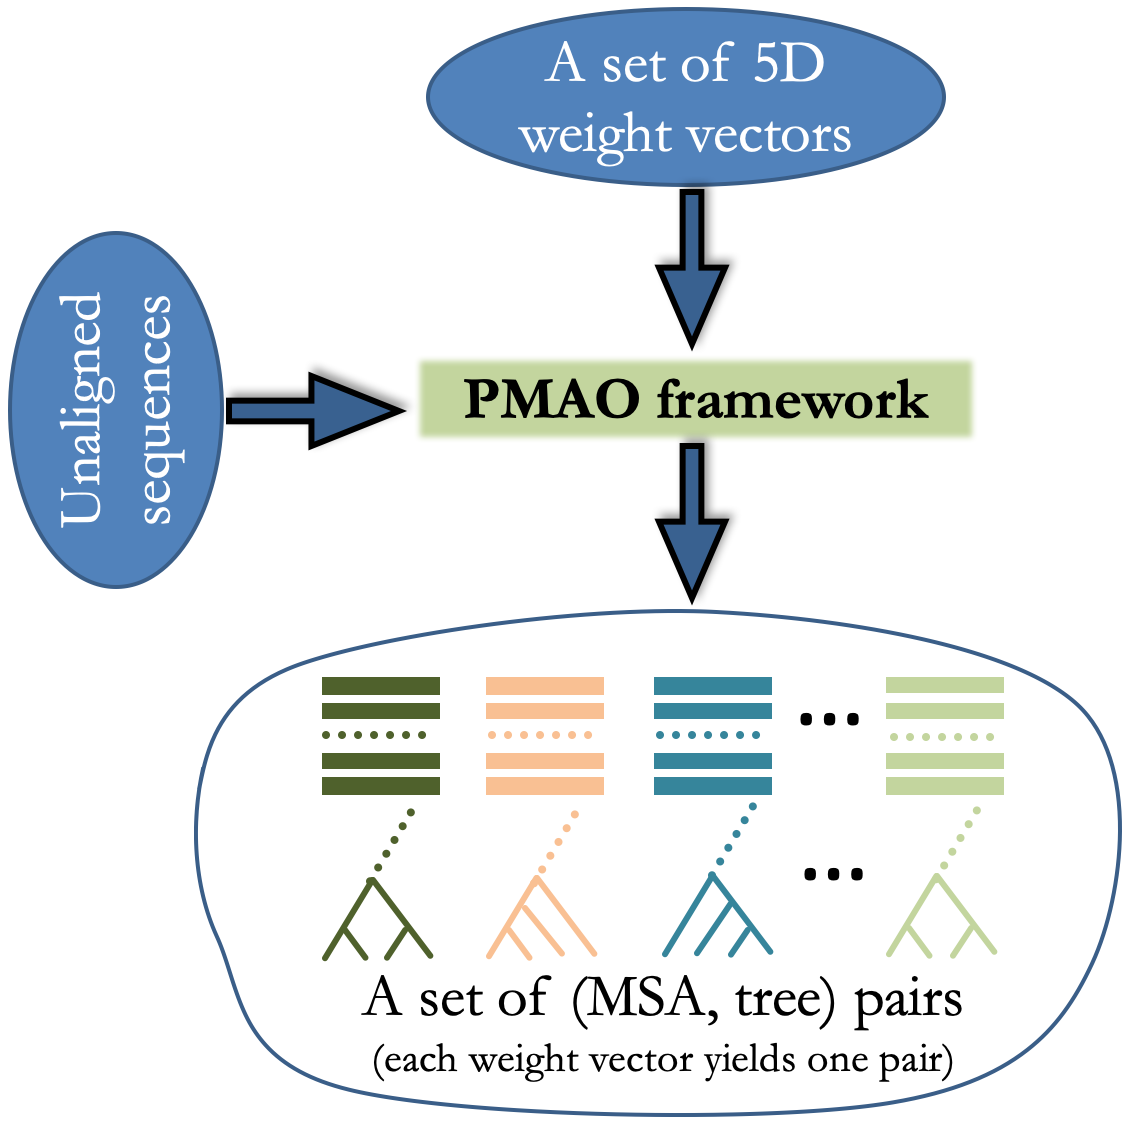
\includegraphics[width=0.28\textwidth]{PMAO}}%
		\subfloat[A high-level workflow for one weight vector]{\label{fig:PMAO:flow}
\colorlet{lcfree}{green}
\colorlet{lcnorm}{blue}
\colorlet{lccong}{red}

% -------------------------------------------------
% Set up a new layer for the debugging marks, and make sure it is on
% top
\pgfdeclarelayer{marx}
\pgfsetlayers{main,marx}
% A macro for marking coordinates (specific to the coordinate naming
% scheme used here). Swap the following 2 definitions to deactivate
% marks.
\providecommand{\cmark}[2][]{%
  \begin{pgfonlayer}{marx}
    \node [nmark] at (c#2#1) {#2};
  \end{pgfonlayer}{marx}
  } 
\providecommand{\cmark}[2][]{\relax} 
% -------------------------------------------------

%\begin{figure}[h]

%\centering
% -------------------------------------------------
% Start the picture
%\subfloat[BB50016]{
\resizebox{0.44\textwidth}{!}{%
\begin{tikzpicture}[%
    >=triangle 60,              % Nice arrows; your taste may be different
    start chain=going below,    % General flow is top-to-bottom
    node distance=6mm and 60mm, % Global setup of box spacing
    every join/.style={norm},   % Default linetype for connecting boxes
    ]
% ------------------------------------------------- 
% A few box styles 
% <on chain> *and* <on grid> reduce the need for manual relative
% positioning of nodes
\tikzset{
  base/.style={draw, on chain, on grid, align=center, minimum height=4ex},
  proc/.style={base, rectangle, text width=19em},
  proc2/.style={base, rectangle, text width=12em},
  test/.style={base, diamond, aspect=2, text width=6em},
  term/.style={proc, rounded corners},
  term2/.style={proc2, rounded corners},
  merge/.style={base, circle},
  % coord node style is used for placing corners of connecting lines
  coord/.style={coordinate, on chain, on grid, node distance=6mm and 25mm},
  % nmark node style is used for coordinate debugging marks
  nmark/.style={draw, cyan, circle, font={\sffamily\bfseries}},
  % -------------------------------------------------
  % Connector line styles for different parts of the diagram
  norm/.style={->, draw, lcnorm},
  free/.style={->, draw, lcfree},
  cong/.style={->, draw, lccong},
  it/.style={font={\small\itshape}}
}
% -------------------------------------------------
% Start by placing the nodes
%\node [proc, densely dotted, it] (p0) {Randomly initialize base locations};
% Use join to connect a node to the previous one 
\node [term, fill=lcfree!25] {Input: unaligned sequences,\\ \scriptsize{$<W_{SIMG},W_{SIMNG},W_{SOP},W_{GAP},W_{ML}>$}};
\node [proc, join] (p0) {$iA \gets$ compute initial alignment\\$iT \gets$ infer ML tree};
\node [proc, join,  fill=lcfree!25] (p01) {$stocDecom \gets False$};
%\node [proc, join] (p1) {$iT \gets$ estimate ML tree};
\node [proc, join, fill=lcfree!25] (p12) {\scriptsize{$SIMG, SIMNG, SOP, GAP, ML \gets$} calculate 5 scores from ($iA, iT$)};
\node [proc, join, , fill=lcfree!25] (p13) {\scriptsize{$bS \gets SIMG \times W_{SIMG} + SIMNG \times W_{SIMNG} + SOP \times W_{SOP} + GAP \times W_{GAP} + ML \times W_{ML}$}};
\node [proc, join] (p14) {($nA, nT) \gets$ run a PASTA iteration to get a new (alignment, tree) pair from ($iA, iT$)\\{~{\footnotesize\ttfamily{/*$stocDecom$  triggers the stochastic decomposition*/}}} };
\node [proc, join, fill=lcfree!25] (p15) {\scriptsize{$SIMG, SIMNG, SOP, GAP, ML \gets$} calculate 5 scores from ($nA, nT$)};
\node [proc, join, fill=lcfree!25] (p16) {\scriptsize{$nS \gets SIMG \times W_{SIMG} + SIMNG \times W_{SIMNG} + SOP \times W_{SOP} + GAP \times W_{GAP} + ML \times W_{ML}$}};
%\node [proc, join, fill=lccong!25, below=1.7cm of p14] (S1) {Update base locations based on current allocations};
%\node [proc, join, fill=lcfree!25, below=1.6cm of S1] (p41) {Calculate allocations for current bases};
%\node [proc, join=by cong]      {Calculate objective with current base locations and allocations};
\node [test,right=6.3cm of p0] (t1) {$(nS > bS)$?};
% No join for exits from test nodes - connections have more complex
% requirements
% We continue until all the blocks are positioned
\node [proc2] (p2) {($bA, bT) \gets (nA, nT)$\\$bS \gets nS$};
\node [proc2, join,  fill=lcfree!25] (p24) {$stocDecom \gets False$};
\node [proc2,  fill=lcfree!25] (p23) {$stocDecom \gets True$};
\node [merge, join] (p21) {};
\node [proc2, join] (p22) {($iA, iT) \gets (nA, nT)$};
% We position the next block explicitly as the first block in the
% second column.  The chain 'comes along with us'. The distance
% between columns has already been defined, so we don't need to
% specify it.
\node [test, join] (t6) {terminate?}; %, right=8cm of S1
%\node [test, join=by free] (t5) {Accept $S_{new}$?};
%\node [proc, join=by free] (p5) {$S_{candidate} \gets S_{new}$};
%\node [proc, join] (p6) {Maintain $S_{best}$};
%\node [proc, join] (p7) {Clear $SEQ$};
%\node [test, join] (t6) {terminate?};
% Some more nodes specifically positioned (we could have avoided this,
% but try it and you'll see the result is ugly).
\node [term2, join] (p10) {Return ($bA, bT$)};
% -------------------------------------------------
% Now we place the coordinate nodes for the connectors with angles, or
% with annotations. We also mark them for debugging.
%DISABLED BY AHMED
\node [coord, right=2.2cm of t1] (c1)  {}; %\cmark{1}   
\node [coord, left=of t6] (c6)  {}; %\cmark{6}   
%\node [coord, right=of t5]  (c8)  {}; %\cmark{5}  
\node [coord, left=of t6, xshift=-17em]  (cS1)  {}; %\cmark{5}  

% -------------------------------------------------
% A couple of boxes have annotations
%\node [above=0mm of S1, it] {(Location step: Heuristic)~~};
%\node [above=0mm of p41, it] {(Allocation step: Exact) };
% -------------------------------------------------
% All the other connections come out of tests and need annotating
% First, the straight north-south connections. In each case, we first
% draw a path with a (consistently positioned) annotation node, then
% we draw the arrow itself.
\path (t1.south) to node [near start, xshift=1em] {$y$} (p2);
  \draw [*->,lcnorm] (t1.south) -- (p2);
%\path (t5.south) to node [near start, xshift=1em] {$y$} (p5); 
%  \draw [*->,lcfree] (t5.south) -- (p5);
\path (t6.south) to node [near start, xshift=1em] {$y$} (p10); 
  \draw [*->,lcnorm] (t6.south) -- (p10);
% -------------------------------------------------
% Finally, the twisty connectors. Again, we place the annotation
% first, then draw the connector
\path (t1.east) to node [near start, yshift=1em] {$n$} (c1); 
  \draw [*->,lcnorm] (t1.east) -- (c1) |- (p23);
  
\draw [->,lcnorm] (p24.west) -- ++(-4mm,0) |- (p21);


\path (t6.west) to node [yshift=-1em] {$n$} (c6); 
  \draw [*->,lcnorm] (t6.west) -- ++(-16mm,0)  |- (p14.east);

% -------------------------------------------------
% A last flourish which breaks all the rules
%\draw [->,MediumPurple4, dotted, thick, shorten >=1mm]
%  (p2.south) -- ++(5mm,-3mm)  -- ++(27mm,0) 
%  |- node [black, near end, yshift=0.75em, it] {SM to SA} (p4);

\draw [->,lcnorm]
  (p16.south) -- ++(5mm,-3mm)  -- ++(31mm,0) 
  |- node [black, near end, yshift=0.75em, it] {} (t1.west);
  
\end{tikzpicture}
}
%}
%\end{adjustwidth}
%\caption{A high-level workflow of PMAO for one weight vector.}
%\label{fig:flowchart}
%\end{figure}

}%
		\subfloat[30 well-spaced 5D weight vectors]{\label{fig:weight}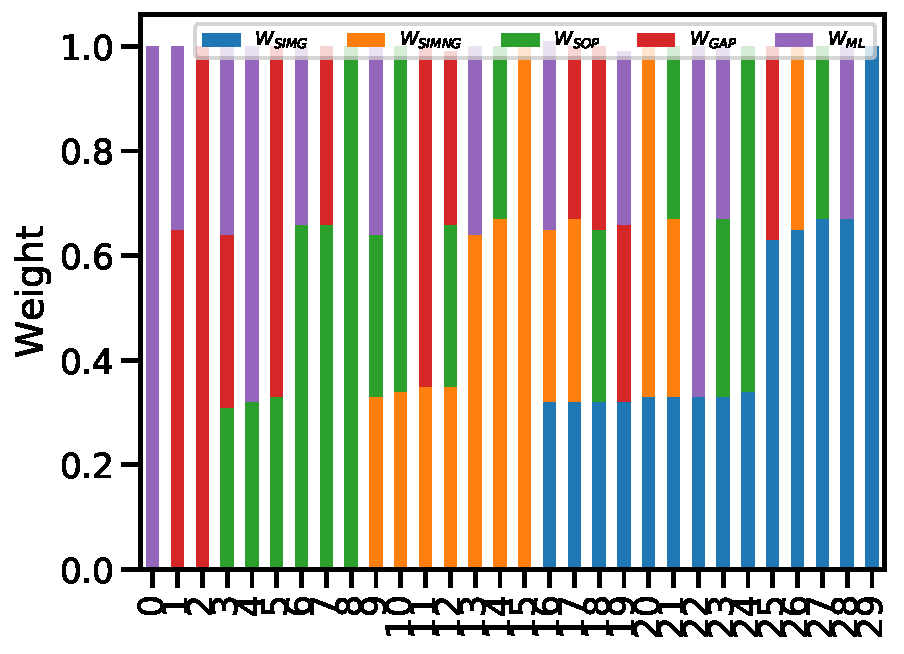
\includegraphics[width=0.35\textwidth]{30-weight.pdf}}
	\end{adjustwidth}
	\caption{A simplified illustration of our PMAO framework.}
	\label{fig:PMAO}
\end{figure*}

\subsection{Application-aware objective functions}
Alongside the ML score, we incorporate the following four simple objective functions, identified by~\cite{nayeem2020multiobjective} based on their better correlation to the tree accuracy, in our PAMO framework. Several pairs of these objectives may have conflicting relationship~\cite{nayeem2020multiobjective}.  
\begin{enumerate}
	\item Maximize similarity for columns containing gaps (SIMG): For each column of the MSA having at least one gap, it calculates the ratio of the most frequent characters. Then all those ratios are added to get the SIMG score.
	\item Maximize similarity for columns containing no gaps (SIMNG): This is similar to SIMG except that it considers those columns of the MSA that do not have any gap.
	\item Maximize sum-of-pairs (SOP): For each pair of aligned sequences in the MSA, it takes the sum of substitution score for the two aligned characters across all columns using a substitution matrix. The addition of all pairwise scores gives the SOP score. In this paper, we use the BLOSUM62 matrix for protein sequences.
	\item Minimize the number of gaps (GAP): The summation of the number of gap characters in each aligned sequence. For the sake of uniformity, we convert this score into a maximization criterion.
\end{enumerate}


\subsection{PMAO framework}
\subsubsection{MO principles}
The goal of an MO algorithm is to generate a set of solutions, popularly known as the Pareto-optimal solutions in the MO literature, which represent the best compromise among the (conflicting) objectives. 
%In the MO literature, these solutions are popularly said to constitute the Pareto front of the solution space. 
Among the several classes of MO algorithms (e.g., pareto-based, decomposition-based, indicator-based, etc.), decomposition-based strategies are found effective to face the difficulties in handling `many' (i.e., more than three) objectives~\cite{li2015many}. These algorithms decompose the task of generating several alternative solutions into many single-objective problems with the help of a set of well-distributed weight vectors, popularly known as reference directions. Each weight vector aggregates the different objective scores into a single value that eventually leads to one member of the final solution set.

\subsubsection{Simplified workflow}
We develop a decomposition-based MO framework, namely, PASTA with many application-aware objectives (PMAO) (Figure~\ref{fig:PMAO}) by driving the search process of PASTA with a total of five objectives directed by a 5D weight vector. Figure~\ref{fig:PMAO:flow} depicts a high-level workflow for one weight vector, where the steps inspired by the MO approach are marked as green. This workflow is executed for all weight vectors to get alternative solutions and can be performed independently in parallel. As will be evident later, PMAO treats a solution better than the other based on the weighted-sum of five objective values instead of using ML score alone. Also, note that PMAO keeps track of whether an improved solution is generated at the previous iteration through a boolean variable \textit{stocDecom}. It impacts the divide-and-conquer strategy within PASTA by enabling the stochastic decomposition, which will be discussed soon. PMAO uses the default behavior of PASTA unless mentioned otherwise.

\subsubsection{Weight vectors}
Although working with a higher number of weight vectors increase the chance of getting better solutions in the solution set, we choose to work with 30 weight vectors to reduce the computational burden as well as to demonstrate the synergy between PASTA and an MO approach since 30 is quite a low number to tackle 5 objectives alone by an MO algorithm~\cite{deb2014evolutionary}. We calculate 30 well-spaced points on a 5D unit simplex using the method suggested by~\cite{ref_dirs_energy} as our weight vectors. Each of the 30 vertical bars in Figure~\ref{fig:weight} depicts one weight vector. %The workflow of

\begin{algorithm}[!htbp]%[!htbp]
	\scriptsize
	\textbf{Input:} $tree$: to be bisected; $maxSize$: max. allowable leaves in a tree; $stocDecom$: triggers the stochastic decomposition 
	%\textbf{Output:} $M$: the modified solution\\
	\begin{algorithmic}[1]
		\caption{min-cluster-size-bisect}
		\label{algo:min-bisect}
		\State{$nodeLeaves \gets$  empty dictionary}
		\For{each node $b$ in post-order-traverse($tree$)}	
		\For{each child $c$ of node $b$}
		\State $nodeLeaves[ch] \gets $ \Call{leaf-count}{$ch$}
		\EndFor 
		\If{ \Call{leaf-count}{$b$} $> maxSize$}
		\If{$stocDecom = False$}
		\State $selected \gets$ the node $x$ with the maximum $nodeLeaves[x]$ value
		\Else	
		\State $selected \gets $ fitness proportionate selection where selection probability of a node $x \propto nodeLeaves[x]$ \Comment{stocastic decompostion} \label{algo:min-bisect:stoc}
		\EndIf
		\EndIf
		\State $t1 \gets $ the subtree of $tree$ rooted at $selected$
		\State remove $selected$ from its parent in $tree$
		\EndFor
		\State \textbf{return} $tree, t1$
		\Statex
		
		\Function{leaf-count}{$node$, $tree$}
		\State $ count $ $\gets$ no. of leaves in the subtree of $tree$ rooted at $node$
		\State \textbf{return} $ count $
		\EndFunction
	\end{algorithmic}
\end{algorithm}

\subsubsection{Stochastic decomposition}\label{subsec:stocastic}
We also enhance PASTA's divide-and-conquer method in the context of MO principles due to its huge impact on the accuracy of the generated (MSA, tree) pair~\cite{liu2012sate}. The heart of this strategy is a decomposition method that divides the leaves (i.e., unaligned sequences) of the guide tree into disjoint subsets. Since version 1.8.0, PASTA has been using \textit{mincluster} decomposition~\cite{balaban2019treecluster} which minimizes the number of resultant subsets given the maximum allowable members in a subset (\textit{maxSize} parameter in Algorithm~\ref{algo:min-bisect}). The default value of this parameter is set to half of the total leaf count. \textit{mincluster} strategy is implemented by repeatedly calling a method, namely, \textit{min-cluster-size-bisect}, to bisect a given tree. Scanning the nodes of the input tree in a post-order manner, it removes the subtree with the maximum number of leaves not exceeding the \textit{maxSize}. We embed some randomness in this method to (i) help PASTA to escape local optima and to (ii) increase the diversity of the solution set generated by PMAO. Line~\ref{algo:min-bisect:stoc} of Algorithm~\ref{algo:min-bisect} enforce the idea of stochastic decomposition, which randomly picks a subtree with the selection probability proportional to the number of leaves under that subtree.

\begin{algorithm}[!htbp]%[!htbp]
	\scriptsize
	\textbf{Input:} $SIMG, SIMNG, SOP, GAP, ML$: scores to be normalized
	%\textbf{Output:} $M$: the modified solution\\
	\begin{algorithmic}[1]
		\caption{rough-normalization}
		\label{algo:normalize}
		\State $GAP \gets 1.0/GAP$ \Comment{convert into a maximiation score}
		\State $ML \gets -1.0/ML$ \Comment{shift the value range to positive zone}
		\State $ obj \gets [SIMG, SIMNG, SOP, GAP, ML]$
		\State $max \gets$ the maximum value in $obj$
		\State $max \gets$ cast $max$ as integer
		\State $d \gets$ the no. of digits in $max$
		\State $ base \gets 10^{d+1}$
		\State add $base$ to all values in $obj$
		\For{$i \gets$ 0 to 4}
		\State $obj[i] \gets $ \Call{softsign}{$obj[i]$}
		\EndFor
		\State \textbf{return} $obj$
		\Statex
		
		\Function{softsign}{$x$} \label{algo:normalize:softsign}
		\State \textbf{return} $ \frac{x}{1 + |x|} $
		\EndFunction
	\end{algorithmic}
\end{algorithm}

\begin{figure}[!htbp]%
	%\centering
	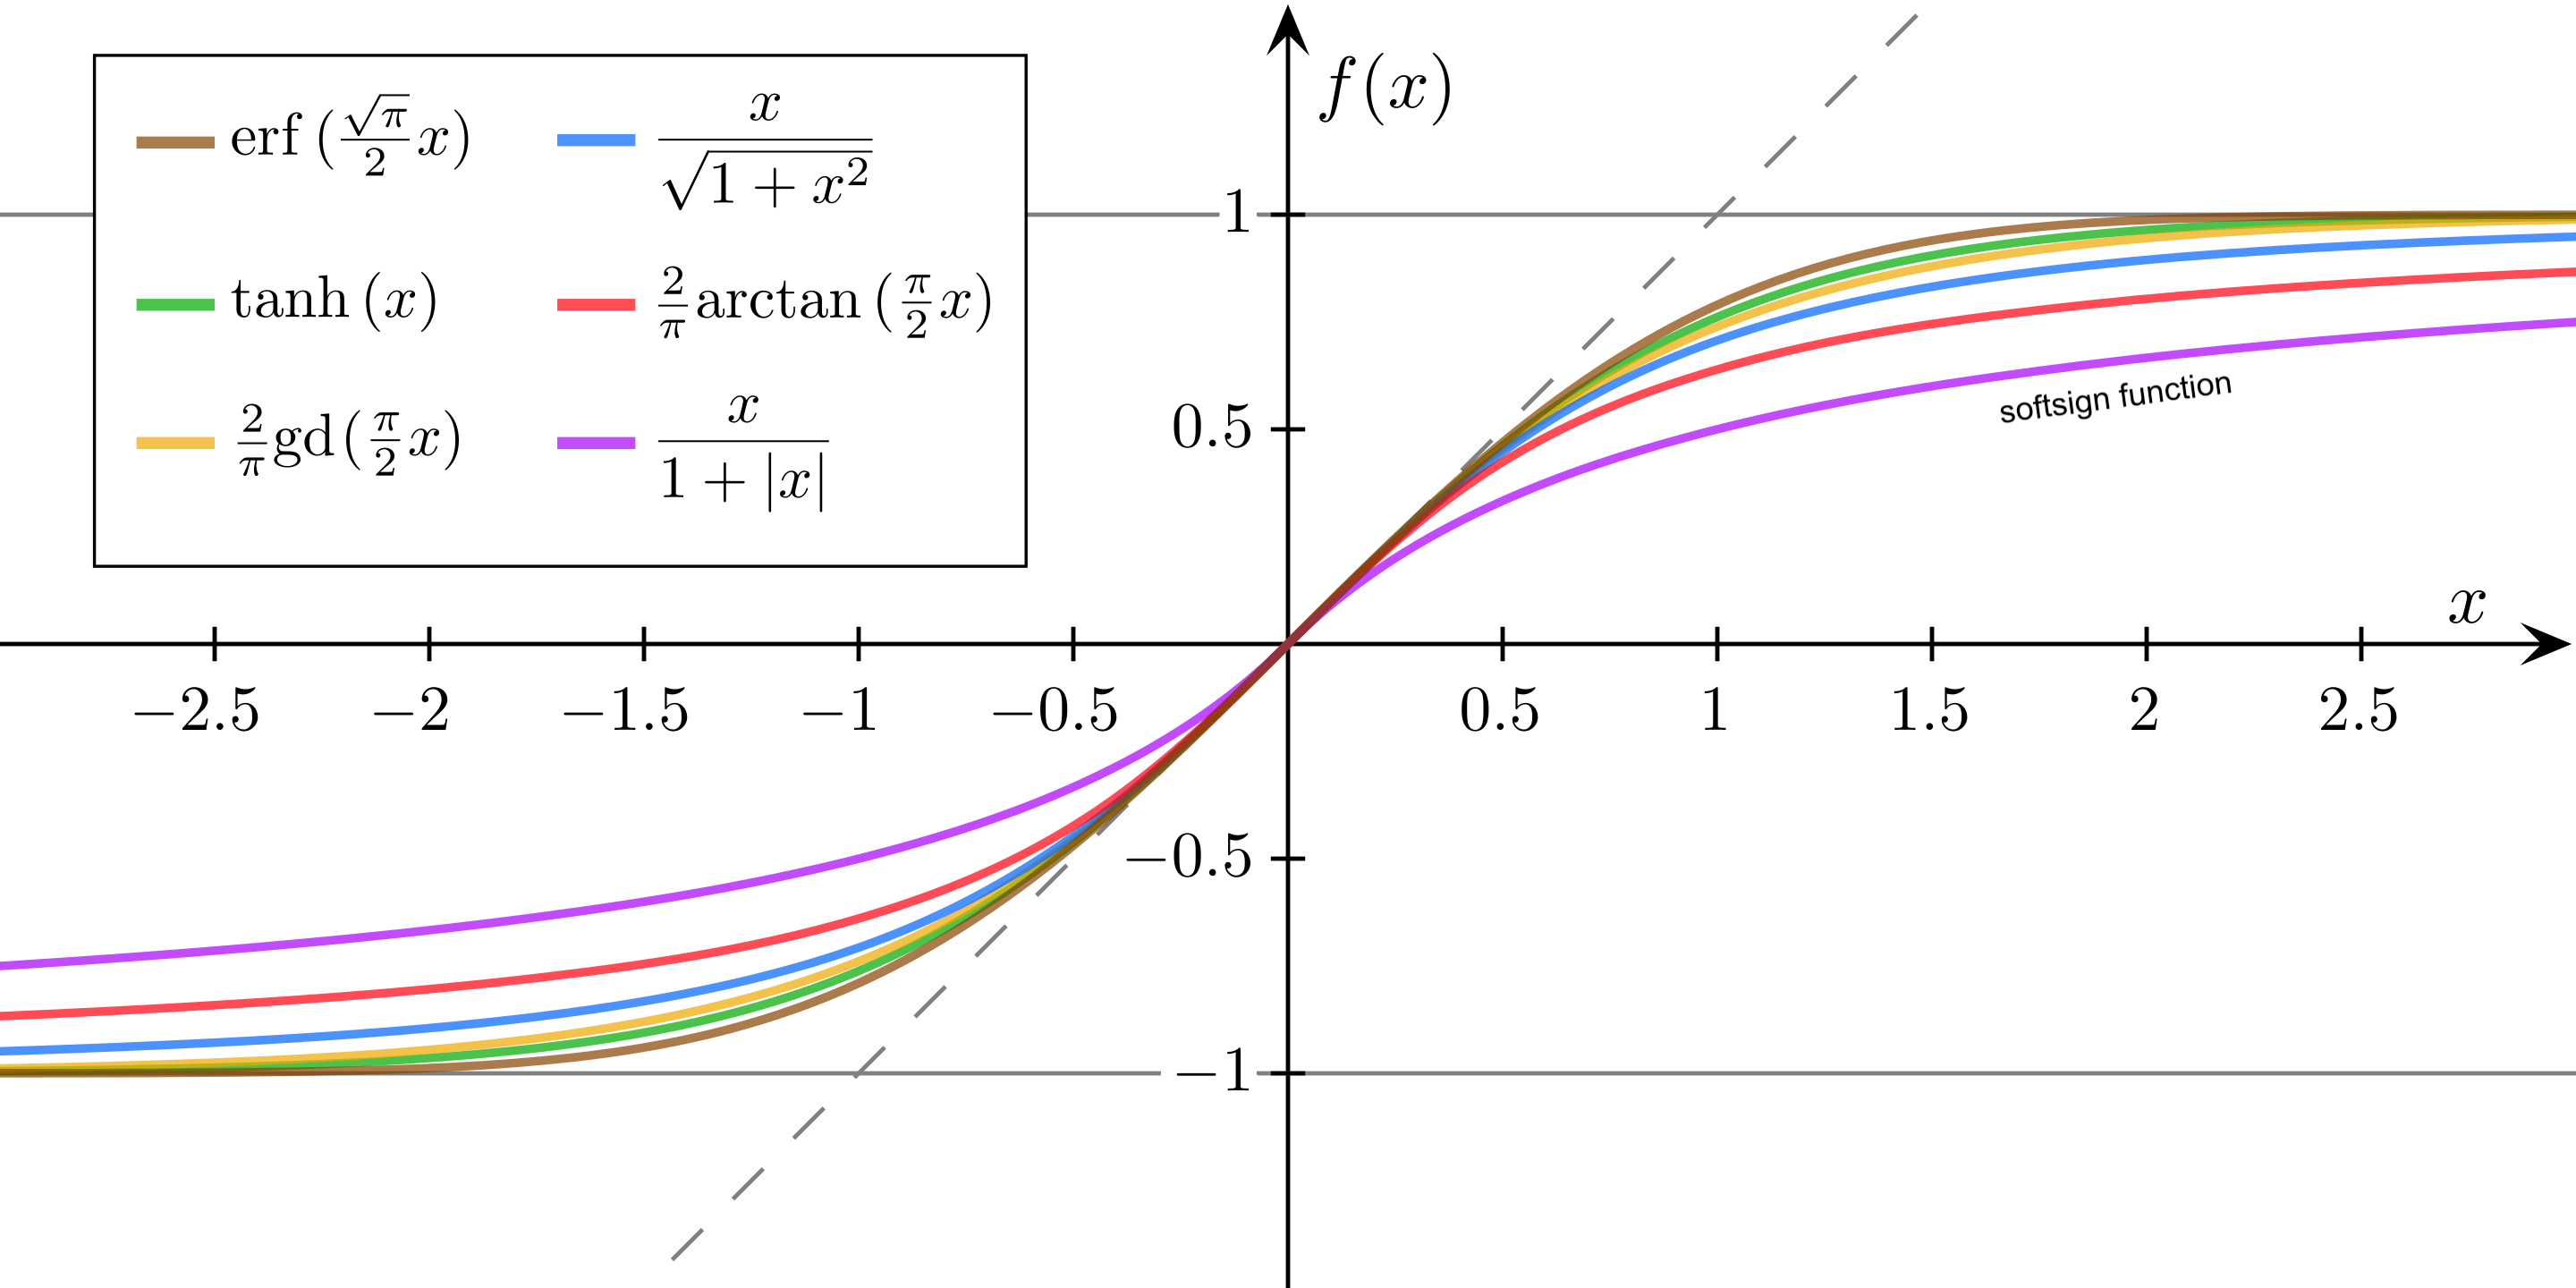
\includegraphics[width=0.4\textwidth]{sigmoid}
	\caption{Some sigmoid functions. Taken from WIKIPEDIA.}
	\label{fig:sigmoid}
\end{figure}

\subsubsection{Normalization}
%Finally, we present the way we overcome a hurdle to ensure the desired effect MO strategy within PMAO. 
Each of the five objective functions is measured using different scales, and their ranges differ to a great extent. So without normalization, their weighted-sum may be unexpectedly biased towards the objectives whose range extends far right, on the real number line, to the others. To add further complication, we do not have enough information regarding those objective values' distribution (e.g., min, max, avg, etc.). So we design a \textit{rough-normalization} method outlined in Algorithm~\ref{algo:normalize} which is called before the aggregation. Here we first transform the objective values to have the equal number of integer digits by adding an offset. Then we apply the softsign function (line~\ref{algo:normalize:softsign}) on each transformed value to make them close to 1.0. We choose the softsign function, over other sigmoid functions (Figure~\ref{fig:sigmoid}), as it converges polynomially (rather than exponentially) which helps to reduce further the risk of the aggregation being unjustly biased towards some objectives. %After applying aforementioned normalization, the weighted-sum of the objective values 


\subsection{Domain-specific performance measure}
As we consider phylogeny estimation as the application domain of MSA, we assess the performance of PMAO solely based on the ML trees from its solution set. Therefore, we evaluate the quality of each ML tree with respect to the true phylogenetic tree
using a widely used measure known as the False Negative (FN) rate. FN rate is the percentage of edges present in the true tree but missing in the estimated tree. So a smaller value of the FN rate
is desirable. Although there are two more common tree error measures: False Positive rate and Robinson-Foulds rate, all of them are identical when the true and estimated trees are
binary~\cite{warnow2017computational} trees, which is the case in this paper.


\subsection{Datasets}
We conduct our experiments on the BAliBASE 3.0 benchmark~\cite{thompson2005balibase} which is the most widely used alignment database of protein families. It provides manually refined reference alignments of high quality based on 3D structural superposition. It has 218 datasets which are organized into six groups according to their families and similarities: RV11
(very divergent sequences, residue identity below 20\%), RV12 (medium to divergent sequences, 20\%-40\% residue identity), RV20 (families with one or more highly divergent sequences), RV30 (divergent subfamilies), RV40 (sequences with large terminal N/C extensions), and RV50 (sequences with large internal insertions). To compare among different variants of PASTA and PMAO, we randomly sample 51 datasets in a stratified way within six groups. We divide them into set A and set B (listed by Table~\ref{tab:balibase}) for ease of presentation. Notably, in this paper we primarily focused on improving the accuracy of PASTA and hence designed our experiments accordingly. We did not experiment scalability by working on larger datasets as PASTA is considered as a highly scalable tool.

\begin{table}[!htbp]
	\scriptsize
	%\centering
	\caption{ Datasets selected randomly from BAliBASE 3.0 benchmark.}
	\begin{adjustwidth}{-0.5cm}{}
	\begin{tabular}{|l|L{3.6cm}|L{3.6cm}|}
		\hline
		\multicolumn{1}{|c|}{Group} & Set A & Set B \\
		\hline
		RV11  & BB11005, BB11018, BB11020, BB11033 & BB11007, BB11019, BB11034, BB11038 \\
		\hline
		RV12  & BB12001, BB12013, BB12022, BB12035, BB12044 & BB12005, BB12026, BB12029,  BB12037\\
		\hline
		RV20  & BB20001, BB20010, BB20022, BB20033, BB20041 & BB20002, BB20012, BB20030, BB20037\\
		\hline
		RV30  & BB30002, BB30008, BB30015, BB30022 & BB30003 BB30011, BB30021, BB30026\\
		\hline
		RV40  & BB40001, BB40013, BB40025, BB40038, BB40048 & BB40006, BB40009, BB40019, BB40033 \\ %
		\hline
		RV50  & BB50001, BB50005, BB50010, BB50016 &  BB50006 BB50002, BB50009, BB50014 \\
		\hline
	\end{tabular}%
	\label{tab:balibase}%
	\end{adjustwidth}
\end{table}%

As we adopt the FN rate as our domain-specific performance measure, following the strategy of~\cite{mirarab2015pasta} we generate a reference tree for each dataset by inferring an ML tree from the reference alignments using RAxML~\cite{stamatakis2014raxml} with bootstrapping and retaining only the highly supported edges. 

%\subsection{Machine learning to predict potential weight vectors}


\begin{comment}

\colorlet{lcfree}{green}
\colorlet{lcnorm}{blue}
\colorlet{lccong}{red}

% -------------------------------------------------
% Set up a new layer for the debugging marks, and make sure it is on
% top
\pgfdeclarelayer{marx}
\pgfsetlayers{main,marx}
% A macro for marking coordinates (specific to the coordinate naming
% scheme used here). Swap the following 2 definitions to deactivate
% marks.
\providecommand{\cmark}[2][]{%
  \begin{pgfonlayer}{marx}
    \node [nmark] at (c#2#1) {#2};
  \end{pgfonlayer}{marx}
  } 
\providecommand{\cmark}[2][]{\relax} 
% -------------------------------------------------

\begin{figure}[h]
\begin{adjustwidth}{-0.6cm}{}	
%\centering
% -------------------------------------------------
% Start the picture
\resizebox{0.55\textwidth}{!}{%
\begin{tikzpicture}[%
    >=triangle 60,              % Nice arrows; your taste may be different
    start chain=going below,    % General flow is top-to-bottom
    node distance=6mm and 60mm, % Global setup of box spacing
    every join/.style={norm},   % Default linetype for connecting boxes
    ]
% ------------------------------------------------- 
% A few box styles 
% <on chain> *and* <on grid> reduce the need for manual relative
% positioning of nodes
\tikzset{
  base/.style={draw, on chain, on grid, align=center, minimum height=4ex},
  proc/.style={base, rectangle, text width=19em},
  proc2/.style={base, rectangle, text width=13em},
  test/.style={base, diamond, aspect=2, text width=6em},
  term/.style={proc, rounded corners},
  term2/.style={proc2, rounded corners},
  merge/.style={base, circle},
  % coord node style is used for placing corners of connecting lines
  coord/.style={coordinate, on chain, on grid, node distance=6mm and 25mm},
  % nmark node style is used for coordinate debugging marks
  nmark/.style={draw, cyan, circle, font={\sffamily\bfseries}},
  % -------------------------------------------------
  % Connector line styles for different parts of the diagram
  norm/.style={->, draw, lcnorm},
  free/.style={->, draw, lcfree},
  cong/.style={->, draw, lccong},
  it/.style={font={\small\itshape}}
}
% -------------------------------------------------
% Start by placing the nodes
%\node [proc, densely dotted, it] (p0) {Randomly initialize base locations};
% Use join to connect a node to the previous one 
\node [term, fill=lcfree!25] {Input: unaligned sequences,\\ \scriptsize{$<W_{SIMG},W_{SIMNG},W_{SOP},W_{GAP},W_{ML}>$}};
\node [proc, join] (p0) {$iA \gets$ compute initial alignment\\$iT \gets$ infer ML tree};
\node [proc, join,  fill=lcfree!25] (p01) {$stocDecom \gets False$};
%\node [proc, join] (p1) {$iT \gets$ estimate ML tree};
\node [proc, join, fill=lcfree!25] (p12) {\scriptsize{$SIMG, SIMNG, SOP, GAP, ML \gets$} calculate 5 scores from ($iA, iT$)};
\node [proc, join, , fill=lcfree!25] (p13) {\scriptsize{$bS \gets SIMG \times W_{SIMG} + SIMNG \times W_{SIMNG} + SOP \times W_{SOP} + GAP \times W_{GAP} + ML \times W_{ML}$}};
\node [proc, join] (p14) {($nA, nT) \gets$ run a PASTA iteration to get a new (alignment, tree) pair from ($iA, iT$)\\{~{\footnotesize\ttfamily{/*$stocDecom$  triggers the stochastic decomposition*/}}} };
\node [proc, join, fill=lcfree!25] (p15) {\scriptsize{$SIMG, SIMNG, SOP, GAP, ML \gets$} calculate 5 scores from ($nA, nT$)};
\node [proc, join, fill=lcfree!25] (p16) {\scriptsize{$nS \gets SIMG \times W_{SIMG} + SIMNG \times W_{SIMNG} + SOP \times W_{SOP} + GAP \times W_{GAP} + ML \times W_{ML}$}};
%\node [proc, join, fill=lccong!25, below=1.7cm of p14] (S1) {Update base locations based on current allocations};
%\node [proc, join, fill=lcfree!25, below=1.6cm of S1] (p41) {Calculate allocations for current bases};
%\node [proc, join=by cong]      {Calculate objective with current base locations and allocations};
\node [test,right=6.3cm of p0] (t1) {$(nS > bS)$?};
% No join for exits from test nodes - connections have more complex
% requirements
% We continue until all the blocks are positioned
\node [proc2] (p2) {($bA, bT) \gets (nA, nT)$\\$bS \gets nS$};
\node [proc2, join,  fill=lcfree!25] (p24) {$stocDecom \gets False$};
\node [proc2,  fill=lcfree!25] (p23) {$stocDecom \gets True$};
\node [merge, join] (p21) {};
\node [proc2, join] (p22) {($iA, iT) \gets (nA, nT)$};
% We position the next block explicitly as the first block in the
% second column.  The chain 'comes along with us'. The distance
% between columns has already been defined, so we don't need to
% specify it.
\node [test, join] (t6) {terminate?}; %, right=8cm of S1
%\node [test, join=by free] (t5) {Accept $S_{new}$?};
%\node [proc, join=by free] (p5) {$S_{candidate} \gets S_{new}$};
%\node [proc, join] (p6) {Maintain $S_{best}$};
%\node [proc, join] (p7) {Clear $SEQ$};
%\node [test, join] (t6) {terminate?};
% Some more nodes specifically positioned (we could have avoided this,
% but try it and you'll see the result is ugly).
\node [term2, join] (p10) {Return ($bA, bT$)};
% -------------------------------------------------
% Now we place the coordinate nodes for the connectors with angles, or
% with annotations. We also mark them for debugging.
%DISABLED BY AHMED
\node [coord, right=2.5cm of t1] (c1)  {}; %\cmark{1}   
\node [coord, left=of t6] (c6)  {}; %\cmark{6}   
%\node [coord, right=of t5]  (c8)  {}; %\cmark{5}  
\node [coord, left=of t6, xshift=-17em]  (cS1)  {}; %\cmark{5}  

% -------------------------------------------------
% A couple of boxes have annotations
%\node [above=0mm of S1, it] {(Location step: Heuristic)~~};
%\node [above=0mm of p41, it] {(Allocation step: Exact) };
% -------------------------------------------------
% All the other connections come out of tests and need annotating
% First, the straight north-south connections. In each case, we first
% draw a path with a (consistently positioned) annotation node, then
% we draw the arrow itself.
\path (t1.south) to node [near start, xshift=1em] {$y$} (p2);
  \draw [*->,lcnorm] (t1.south) -- (p2);
%\path (t5.south) to node [near start, xshift=1em] {$y$} (p5); 
%  \draw [*->,lcfree] (t5.south) -- (p5);
\path (t6.south) to node [near start, xshift=1em] {$y$} (p10); 
  \draw [*->,lcnorm] (t6.south) -- (p10);
% -------------------------------------------------
% Finally, the twisty connectors. Again, we place the annotation
% first, then draw the connector
\path (t1.east) to node [near start, yshift=1em] {$n$} (c1); 
  \draw [*->,lcnorm] (t1.east) -- (c1) |- (p23);
  
\draw [->,lcnorm] (p24.west) -- ++(-4mm,0) |- (p21);


\path (t6.west) to node [yshift=-1em] {$n$} (c6); 
  \draw [*->,lcnorm] (t6.west) -- ++(-16mm,0)  |- (p14.east);

% -------------------------------------------------
% A last flourish which breaks all the rules
%\draw [->,MediumPurple4, dotted, thick, shorten >=1mm]
%  (p2.south) -- ++(5mm,-3mm)  -- ++(27mm,0) 
%  |- node [black, near end, yshift=0.75em, it] {SM to SA} (p4);

\draw [->,lcnorm]
  (p16.south) -- ++(5mm,-3mm)  -- ++(31mm,0) 
  |- node [black, near end, yshift=0.75em, it] {} (t1.west);
  
\end{tikzpicture}
}
\end{adjustwidth}
\caption{A high-level workflow of PMAO for one weight vector.}
\label{fig:flowchart}
\end{figure}


\begin{figure}%
%\centering
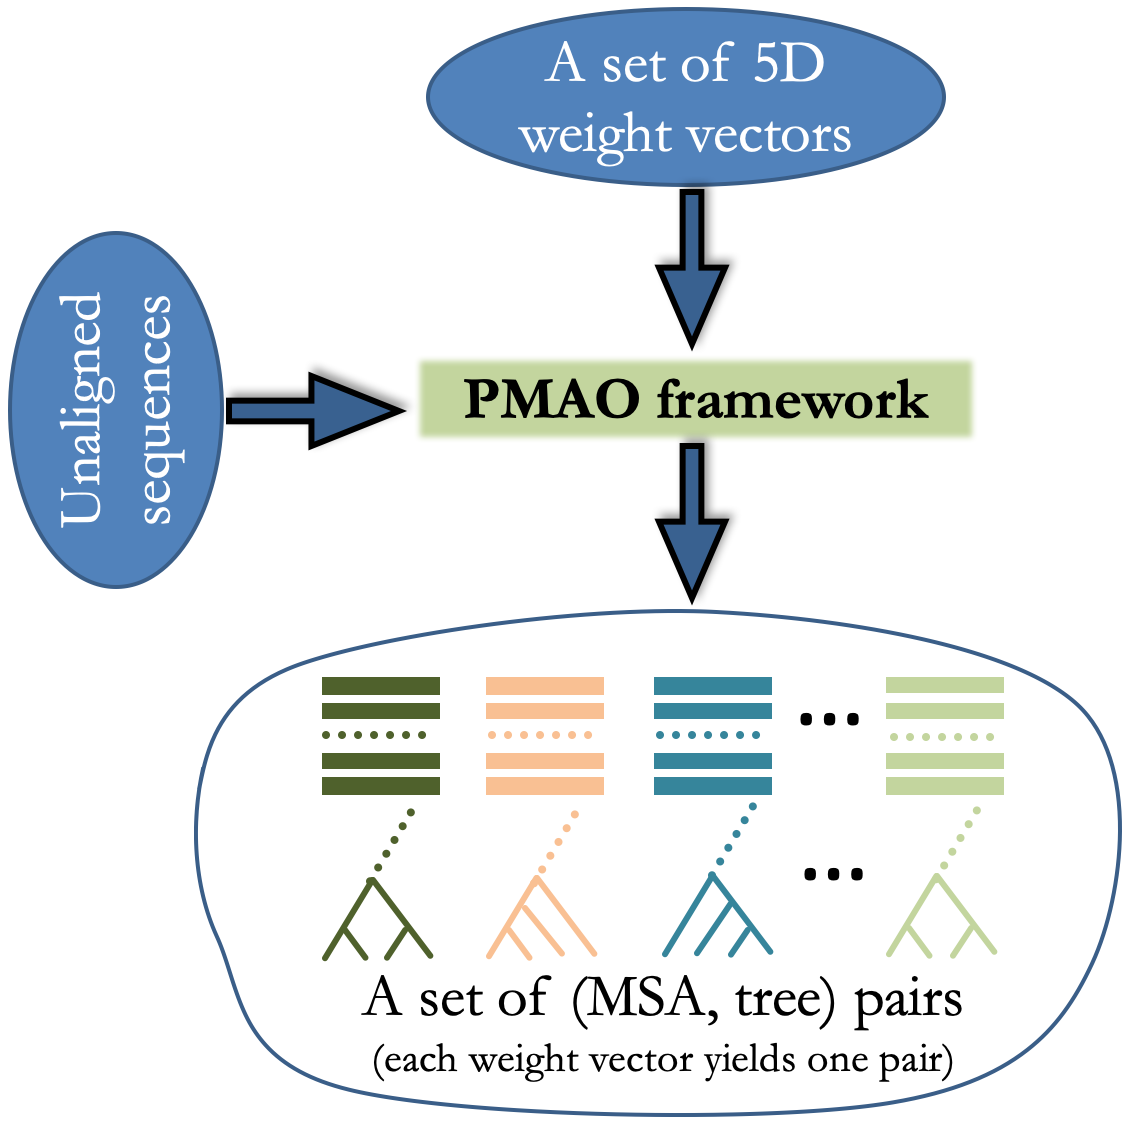
\includegraphics[width=0.35\textwidth]{PMAO}
\caption{Input-output of PMAO framework.}
\label{fig:PMAO2}
\end{figure}
\begin{figure}%
%\centering
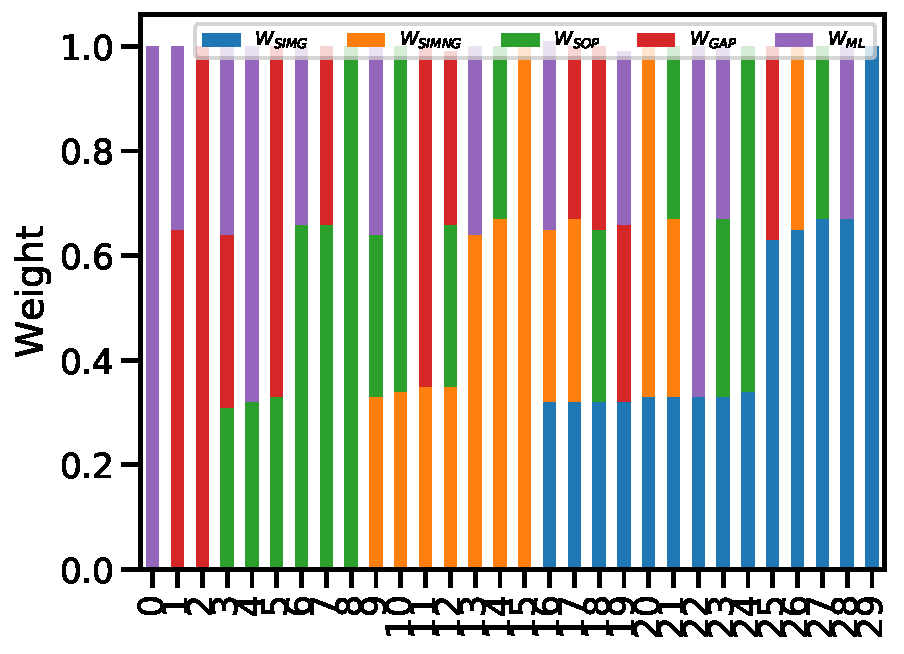
\includegraphics[width=0.45\textwidth]{30-weight.pdf}
\caption{30 well-spaced weight vectors.}
\label{fig:weight}
\end{figure}
\end{comment}